\documentclass[norsk]{article}
\usepackage[norsk]{babel}
\usepackage{amsmath}
\usepackage{gensymb}
\usepackage{parskip}
\usepackage{booktabs}
\usepackage{adjustbox}
\usepackage{tikz}
\usepackage{graphicx}
\usepackage{array}
\usepackage{helvet}
\usepackage{textcomp}
\usepackage{csquotes}
\usepackage{dirtytalk}
\renewcommand{\familydefault}{\sfdefault}
\renewcommand{\baselinestretch}{1.15}



\begin{document}
\renewcommand{\thefootnote}{\roman{footnote}}
\title{TIØ4252 Teknologiledelse - Øving 2}
\author{}
\date{03.10.2019}

\begin{titlepage}
   \begin{center}
 
        \textbf{\huge TIØ4252 Teknologiledelse}\\
        \vspace{4cm}
        \textbf{\huge Øving 2}\\
        \vspace{0.5cm}
        \textbf{\small Gruppe 1, parallell 2}
        
        \vspace{5cm}
        
        \textbf{\small\\*Christopher Janjua\\* }
        \textbf{\small\\*Erlend Marius Ommundsen\\* }
        \textbf{\small\\*Peder Solheim\\* }
        \textbf{\small\\*Runar Sæther\\* }
        \textbf{\small\\*Sivert Laukli\\* }
        
        \vspace{1cm}
 
        
\includegraphics[width=0.4\textwidth, draft=false]{Vedlegg/ntnuLogo.png}
 
        03.10.2019
 
   \end{center}
\end{titlepage}

\newpage
\section{Organisasjonsstruktur}

\subsection{Teori}
De vertikale samordningsmekanismene håndterer behovet for samordning mellom de ulike nivåene i et selskaps hierarki. De skal hovedsakelig sørge for at informasjon mellom ledere og ansatte flyter fritt.

De horisontale samordningsmekanismene skiller seg fra de vertikale ved å fokusere på koordinering mellom de på samme nivå i hierarkiet i bedriften. Her er målet i korte trekk å sørge for at dobbelt arbeid ikke oppstår blant de ansatte.

Fra Henry Mintzbergs modell blir det beskrevet fem måter å samordne på. 

Prosesskontroll handler om å optimalisere arbeidsprosessene, ofte ved å redusere slakk. Et selskap som bruker denne typen kontroll trenger ikke like mye kompetanse, da den ansatte skal gjøre en veldig begrenset og konkret oppgave som en prosessingeniør har delt opp. 

Ved resultatkontroll vurderes resultatet av arbeidet som er blitt utført. Det gir de ansatte muligheten til å jobbe på sin foretrukne måte, få utnyttet sin kompetanse bedre og dermed få økt motivasjon. Ulempene med resultatkontroll er mindre oversikt for lederne og at den er tillitsbasert. Det åpnes heller ikke for dialog om potensiell prosessforbedring. 

\subsection{Nordvest-bygg AS}

Casen om Nordvest-bygg tar for seg et byggeselskap med opprinnelse i Ålesund. Det blir sett på selskapets ekspansjon fra å drive med renovering, til å utvide sitt kompetansegrunnlag ved å påta seg bygging av nybygg.

Nordvest-bygg opplevde en voldsom ekspansjon over en kort tidsperiode. Dette førte til at den vertikale samordningen begynte å slå sprekker. Første omorganisering måtte til da bedriften hadde problemer med å tilpasse organisasjonen med det stadig større antall ansatte. Allerede her ble det tatt valg som fikk konsekvenser for bedriften frem i tid. Hver av de fusjonerte avdelingene fungerte nå som autonome enheter som styrte seg selv og som hadde egne avtaler. 
En slik oppdeling vil gi ledelsen mindre oversikt over hva som faktisk foregår innad i avdelingene, og sier mer om at ledelsen ønsker resultater. Man ser allerede her at sterkere vertikale samordningsmekanismer trengs.

Etter ekspansjonen gikk bedriften inn i en konsolideringsfase, og da spesielt i forbindelse med arbeidsmiljøet. En arbeidsmiljøkomité, som besøkte byggeplasser og regionskontor for å ha samtaler med ansatte, ble dannet. Det kommer frem at de hadde samtaler med over halvparten av alle ansatte. Disse samtalene er et eksempel på fornuftig bruk av vertikal samordning, da det knyttes bånd mellom de ansatte på de forskjellige nivåene i hierarkiet, og ledelsen vil få et bedre innblikk i hva som foregår på de lavere nivåene.

Etter konsolideringsfasen solgte eierne seg ut til et større nasjonalt selskap med store summer til grunn, og bedriften gikk helt bort fra det den stod for med de gamle eierene. En ny eier kom inn i avdelingen som tidligere var Nordvest-bygg og etter en ny omorganisering begynte ansatte å sluntre unna prosjekter med mye reising. Dette er en direkte negativ konsekvens av resultatkontroll, hvor ledelsen i dette tilfellet fokuserte på det ferdige resultatet i motsetning til veien dit. Unnasluntringen førte til sparking av ansatte og prosjektledere, og skapte en nærmest krigstilstand mellom leddene vertikalt i hierarkiet. Altså er dette et tydelig eksempel på problematisk bruk av vertikal samordning.

\subsection{Stol AS}
I casen om Stol beskrives utviklingen av en møbelfabrikk, som startet i det små med utviklingen av stoler basert på en fersk patent på et stivere laminat, og utviklet seg i korte trekk ved å innlemme lokale produsenter av råmateriale fra området rundt til å bli en aktør på flere segmenter av møbelmarkedet.

Parallelt med ekspansjonen av selskapet beskrives også voksesmertene for organisasjonsstrukturen. Ekspansjonene skjedde over kort tid, og ledelsen i selskapet måtte stadig gjøre endringer for å optimalisere produksjonen og overleve.

Da gründeren, Mikal Hansen, døde i 1967, var bedriften midt i en utviklingsprosess av en ny teknisk løsning for laminatet brukt i stolene. Stol mistet dermed pådriveren i selskapet, som de erstattet med den ferdigutdannede maskiningeniøren Torstein Varhei. En av de første endringene Varhei innførte var jobbrotasjon på produksjonslinjene. Dette betydde at alle ansatte måtte lære seg tre arbeidsstasjoner. Som et resultat av denne endringen fikk de ansatte en mer variert arbeidshverdag og det ble lettere å finne en midlertidig erstatter til syke ansatte. Jobbrotasjonen og en reduksjon på antall ansatte per avdeling og økning av antall avdelinger førte til slutt til økt kvalitet i produksjonen. Dette er et eksempel både på god horisontal samordning og prosesskontroll.

\subsection{Vest-Regnskap AB}
Vest-Regnskap AB ble stiftet som et tradisjonelt regnskapsbyrå i 1976, men ble som følge av Monika Halléns innsats et firma som ga unge foreldre en mulighet til å få jobberfaring samtidig som det ga dem tid til å være hjemme med barna. Dette klarte de ved å være basert på deltidsstillinger. 

Mot slutten av casen etter fusjonen med Roger Mostrøms konsulentselskap, oppstod det splid mellom personalansvarlig Mette Zetterlund, daglig leder Mats Johansson og lederen av Malmø-avdelingen, Roger Mostrøm. Da Mostrøm forkastet Zetterlunds forslag om å ta inn deltidsarbeidende i Malmø, gikk Zetterlund til Johansson og fikk ham til å snakke med Mostrøm. Da Zetterlund spurte Johansson om saken i ettertid, fikk hun intet klart svar. Zetterlund fikk deretter et brev som sa at personalansvaret for Malmø-avdelingen nå var Mostrøms, og at all kommunikasjon med ham skulle skje gjennom Johansson. Denne kommunikasjonsprosessen er et eksempel på dårlig horisontal samordning. Ikke bare følger det en forverring av forholdet mellom Zetterlund, Johansson og Mostrøm, men også at kommunikasjonen vil gå tregere mellom partene på grunn av den ekstra forsinkelsen gjennom Johansson.  

\newpage
\section{Ledelse og motivering av ansatte}
\subsection{Teori}

Herzberg tofaktorteori hevder at det er to grupper av faktorer som påvirker motivasjon, hygienefaktorer og motivasjonsfaktorer. Motivasjonsfaktorer kan øke trivsel, i motsetning til hygienefaktorer som kun kan bidra til å hindre mistrivsel. Hygienefaktorer må være tilstede i en tilstrekkelig mengde i et arbeidssystem for å unngå at ansatte blir fraværende. Med hygiene menes det noe som må opprettholdes kontinuerlig.

\vspace{1cm}
\begin{center}
    {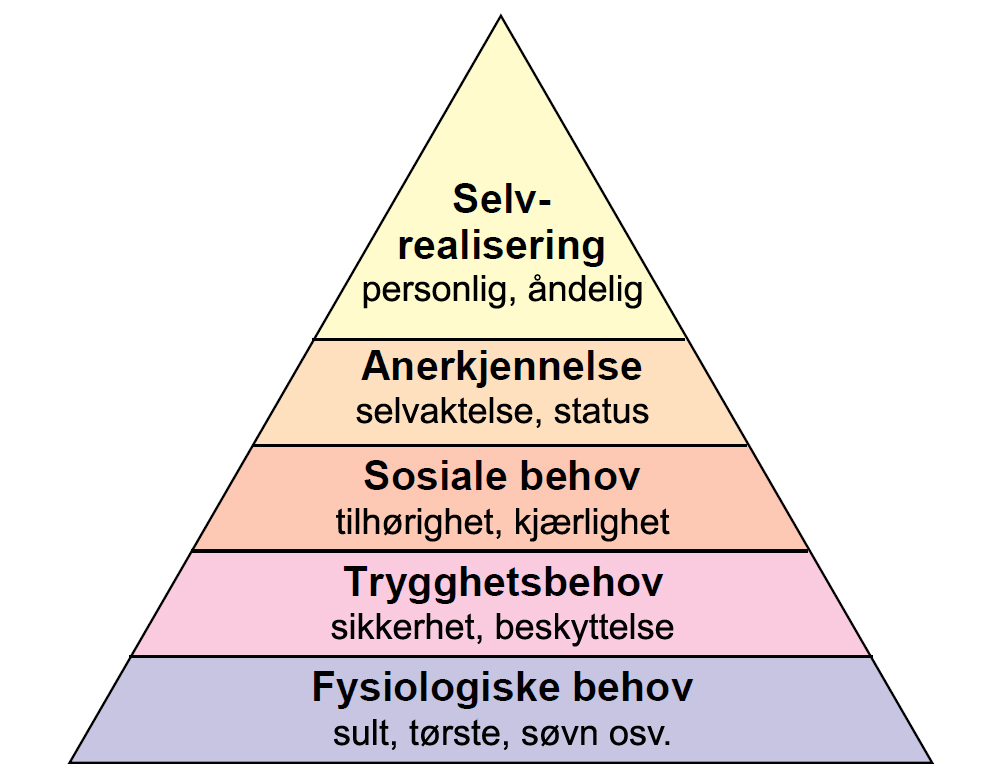
\includegraphics[width=0.6\textwidth, draft=false]{Vedlegg/maslows.jpg}}
\end{center}

\vspace{1cm}

Maslows behovshierarki fremstiller en modell av det Maslow mente var den hierarkiske organiseringen av de behovene vi mennesker har for å fungere. Organisering er lagt med basisbehovene i de nederste lagene. Dersom en streber med å oppfylle et av de nedre lagene, vil en bruke tid på å bekymre seg for å oppfylle et lag som ligger høyere.   

En annen modell som kan brukes for å begrunne motivasjon er Vrooms forventningsteori. Vroom bruker valens for å beskrive hvilke motivasjonsfaktorer som er viktigst for den enkelte verdien som er tilknyttet en belønning.

\vspace{1cm}
\begin{center}
    {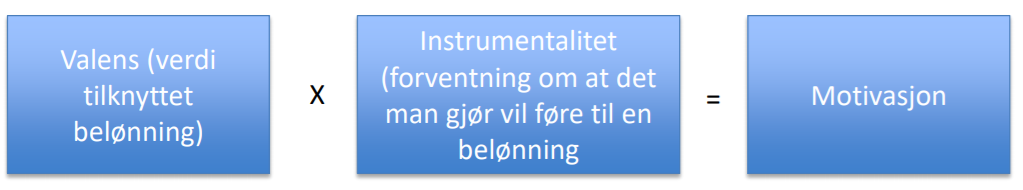
\includegraphics[width=1\textwidth, draft=false]{Vedlegg/Vroom.png}}
\end{center}

\vspace{1cm}

Motivasjonsfaktorene bestemmes av arbeidsgiver her, mens arbeidstaker har selv å bestemme valens på disse faktorene.

\subsection{Nordvest-Bygg AS}

I etterkant av ekspansjonen sin, endret bedriften fokus til arbeidsmiljøet. De visste at vekst og endringer hadde skjedd raskt og at det derfor var et behov for å tilpasse bedriften tilsvarende. En trivselundersøkelse viste at de elementene som skapte stor påkjenning for ansatte var reisingen og ukependlingen mellom hjem og byggeplass. Mange av de ansatte var bekymret for ulykker på grunn av sikring av stillaser, heiser og kraner. Undersøkelsen viste også at de ansatte var fornøyd med lønning og arbeidsoppgaver. Bedriften opprettet en arbeidsmiljøkomité som la frem rapport basert på antall reisedager, pendlerdager, ulykkesstatistikk, og samtaler med opp imot 200 ansatte. 

Rapporten gjorde at Nordvest-Bygg valgte å gjøre innkjøp av bedre møbler og utstyr til brakkebyene hvor de ansatte bodde. De setter opp muligheter for besøk av familie og bedre rotasjon blant hvem som reiser når og hvor de reiser. De reduserer antall ulykker ved hjelp av økte sikkerhetsrutiner. Dette er flere punkter som går under gruppen hygienefaktorer i Herzberg tofaktorteori. Bedre møbler og utstyr i brakkebyene, samt færre reisedøgn og redusert antall ulykker fører til økt trivsel hos ansatte, er arbeidsbetingelser inngår som en av hygienefaktorene. Økte muligheter for besøk fra familie, delvis på bekostning av bedrift, kan minke mistrivsel da mellommenneskelige relasjoner er en hygienefaktor. Så i henhold til Herzberg tofaktorteori var viktige hygienefaktorer fraværende i arbeidsmiljøet i bedriften, noe som skapte mistrivsel hos de ansatte.

De ansatte var allerede fornøyd med arbeidsoppgavene og lønnen. Dette er motivasjonsfaktorer som ikke var fraværende. For at disse motivasjonsfaktorene skulle få best uttelling så måtte hygienefaktorer være på plass og opprettholdt kontinuerlig, noe Nordvest-Bygg gjorde på en god måte. Dette ser vi ut ifra følgende beskrivelse fra casen:

\say{... ting roet seg i bedriften, og siden tidene var gode kunne Nordvest-Bygg fortsette som før i noen år frem til 1997}

Med alle de nevnte tiltakene Nordvest-Bygg gjorde for sine ansatte, oppfylte de også kravene i Maslows behovspyramide på en bedre måte. Selvsagt har alle de ansatte en fast lønn som går både under fysiologiske behov og trygghetsbehov. Uten denne lønnen kan ikke de ansatte dekke sine grunnbehov som mat og drikke. Deres faste lønn kombinert med jobbtrygghet er med på å dekke deres trygghetsbehov. I tillegg oppgraderte Nordvest-Bygg, som nevnt tidligere, sine sikkerhetsrutiner. Dette medførte en halvering av ulykker og nestenulykker på byggeplassene deres. Igjen vil trygghetsbehovet til de ansatte bli ytterligere dekket. Det neste steget i pyramiden er sosiale behov. Under Nordvest-Byggs ekspansjon ble bedriften delt opp i flere kontorer. Dermed ble den ellers tett knyttede arbeidsstokken tvunget til å reise mer. For å opprettholde det gode sosiale miljøet, ble arbeidsstokken delt inn i arbeidslag som skulle reise og jobbe sammen. Nordvest-Bygg gjorde med andre ord flere gode inngrep for å dekke de tre nederste behovene i Maslows behovspyramide. Uten disse som et grunnlag, ville det blitt for vanskelig å dekke de andre behovene.

\subsection{Bjørnsen og Sønn Støperier}
Bjørnsen og Sønn Støperier ble stiftet i 1924 og måtte vente lenge før de på slutten av 70-tallet ble et markedsledende støperi i Norge. Mye av grunnen til at de ble det var at Torbjørn Bjørnsen, eldstesønn av stifteren Bjørn Bjørnsen, ble daglig leder. Bjørnsen ønsket å fokusere på tre elementer: oppgradering av utstyr, heving av ansattes kompetansenivå og restrukturering av kundemassen. Det viste seg å være en nøkkel til suksess for støperiet. Når det kommer til hevingen av kompetansenivå, kan vi se at Vrooms forventningsteori ble tatt i bruk. Bjørnsen oppfylte de ansattes krav om mer lønn dersom de tilegnet seg den nye kompetansen. De som valgte å ikke gjøre det, skulle likevel ikke få sparken. Ettersom de fleste økte kompetansen, anså de ansatte en lønnsøkning som en verdifull belønning. De ansatte visste også at de kom til å få lønnsøkningen, fordi det var deres forslag, og det var godkjent av Bjørnsen. Alt dette førte til at arbeiderne ble motiverte, og ifølge casen ble det stor entusiasme rundt kursene. 

\newpage
\section{Teamarbeid}

\subsection{Teori}
Et team kan beskrives som en gruppe av to eller flere personer som er satt sammen for å nå et felles mål over en gitt tidsperiode. Teammedlemmene har delte normer for hvordan oppgaver skal løses for nå målet.

Kommunikasjon er essensielt for etablering og utvikling av team. Hvis ikke alle teammedlemmer føler seg lyttet til, vil de føle et ubehag og videre engasjering blir problematisk. Dette fører til ineffektiv kommunikasjon og dermed ineffektivt teamarbeid.

MRPI-modellens består av fire punkter. Et punkt er avklaring av mål. Her er det viktig at alle teammedlemmer får samme oppfatning av hva målet er med en klar og presis målformulering. Et annet punkt er prosedyrer. Her inngår regler, normer og rutiner for hvordan teamarbeidet skal fungere fra dag til dag. Spørsmål som må besvares under dette punktet er blant annet hvordan beslutninger skal tas, hvordan arbeidsoppgavene skal fordeles og hvordan teamet skal takle eventuelle konflikter.

\subsection{Nordvest-Bygg AS}

Åge ble satt til å være leder i en nydannet arbeidsmiljøkomité. Denne komiteen ble sammensatt for å forbedre arbeidsmiljøet for de ansatte. De mente ulykkesstatistikken innen de ulike byggeprosjektene var for høye, og den endrede markedsstrukturen førte til flere reisedager. Komiteen hadde felles mål i å både redusere ulykkesstatistikken til et minimum, men også å øke trivsel hos de ansatte. Arbeidet deres gikk ut på å kommunisere mellom ansatte og ledelse for å komme frem til ulykkesreduserende tiltak.

Opprettelsen av komiteen er et godt håndtert aspekt i henhold til teamarbeid i bedriften. Komiteen er et eksempel på et team, da alle deltakerne har et felles konkret mål de ønsker å nå innenfor en gitt tidsperiode. I henhold til MRPI-modellen er en god målformulering og en felles forståelse for denne en stor faktor for at samarbeid innad i teamet fungerer bra og for at unødvendige konflikter ikke oppstår.

I etterkant av eierskapskifte finner vi eksempler på dårlig håndterte aspekter. Da Nordvest-Bygg ble kjøpt opp av Norgesbygg, kom Georg inn som ny leder. Han satte sammen et team for å gjennomføre ønskene fra ledelsen om å omstrukturere selskapet. De øvrige teammedlemmene hadde jobbet sammen i lang tid og hadde allerede skapt tillit til hverandre, samt utviklet felles normer og regler for teamarbeidet. Georg kom inn som et nytt medlem uten forståelse for teamets normer. Det nye sammensatte teamet fikk trolig ikke nok tid til å etablere et grunnlag for å bygge tillit med sitt nye medlem. Det virket til at Georg ønsket å gjennomføre de strukturelle endringene så hurtig som mulig, etter press fra hovedkontoret.

Et par av de ønskede endringene ble møtt med hard motstand og ble forkastet. Det ene endringsønsket var å sette inn en prosjektbasert matrise, som hadde som mål om å bedre utnytte arbeidskapasiteten som var tilgjengelig. Dette ble innført i strid med hva de andre teammedlemmene mente. Hovedargumentet var at denne endringen ville føre til økt antall reisedager, som var lite ønskelig. Siden Georg ikke lenger kom til enighet med medlemmene, kan det se ut til at dette er en kommunikasjonssvikt innad i teamet. Dette er et eksempel på et dårlig håndtert aspekt. Uten riktig kommunikasjon vil beslutningsprosessen bli vanskelig. De øvrige teammedlemmene føler seg lite lyttet til og ikke inkludert. Dermed blir videre engasjering vanskelig. Dette gjør det enda lettere for Georg å ta beslutninger for seg selv, og konturene av et team blir svakere.

Prosedyrepunktet i MRPI-modellen understreker at beslutningsprosessen også er et dårlig håndtert aspekt. Her er det flere underpunkter som ikke er fulgt. Teamet har ikke blitt enige på forhånd om hvordan beslutninger skal tas eller hvordan de skal takle eventuelle konflikter. Dette fører til at teamstrukturen går i oppløsning, da de ikke har noen oppfatning av hvilke felles regler og normer som gjelder, som er et nøkkelpunkt for at teamet skal bli vellykket. 

\newpage
\section{Den norske modellen}

\textbf{Eksempel fra Nordvest-Bygg AS:}

\say{Åge ble dermed leder for den nye arbeidsmiljøkomiteen, der det også deltok to andre representanter for ledelsen samt to representanter fra fagforeningen. Komiteen reiste rundt på ulike byggeplasser samt regionskontorene og hadde samtaler med de ansatte, og la etter ett års arbeid frem en rapport for styret.}

\textbf{Eksempel fra Tungesvik Stålsveis AS:}

\say{Bedriften har en annen gruppe på 3 ansatte som er avsatt til å drive vedlikehold på trålerne. Disse administrerer seg selv, og leverer timelister og lister over materialforbruk direkte til Jan}

Den norske modellen er tilpasset for å fellesoptimalisere produktivitet, arbeidsmiljø og industrielt demokrati. I treparts-samarbeidet fungerer et samarbeid mellom staten, lederskapet i bedriften og tillitsvalgte. Målet er å oppnå økt verdiskapning gjennom bred medvirkning\cite{torvatn}. De ansatte har ved loven rett til å medvirke til avgjørelser som blir tatt i bedriften. I forhandlinger og samarbeid med ledelsen er de ansatte representert av tillitsvalgte. I det første eksempelet over skal Nordvest-Bygg overkomme utfordringer med å ha mye reisevirksomhet. Det settes sammen en komité med representanter fra ledelsen og tillitsvalgte. Noe som er karakteristisk for samarbeidsmodellen. Ved å involvere de tillitsvalgte i undersøkelsene av arbeidsmiljøet sørger bedriften for at de ansattes interesser er med på utformingen av løsningen. Dermed kan de komme frem til en konstruktiv løsning som har forankring blant de ansatte. Slik kan de unngå konflikt. 

Hva om lederne i Nordvest-Bygg hadde utviklet en løsning uten medvirkning fra de ansatte? Det kan tenkes utvikling av en slik løsning ville foregått med mindre grad av oversikt over tilstander som angår de ansattes behov. Det kan være fare for at avgjørelsene som blir tatt utvikles utelukkende med hensyn til å øke profittmarginer. En slik løsning kan gå på bekostning av arbeidsmiljøet og skape mistrivsel blant ansatte. Dette kan forårsake utvikling av nye konflikter og problemer. På den måten kan en se på trepartsamarbeidet som et preventivt virkemiddel.  

Hvilke ulemper kan representativ medvirkning medbringe? Dette kan føre til utvikling av nye konflikter. På den måten kan en se på trepartssamarbeidet som et preventivt virkemiddel. Hvilke ulemper kan representativ medvirkning medbringe? I representativ medvirkning er tillit mellom de tillitsvalgte og de ansatte sentralt. Det er fare for at tillit blir misbrukt. Det er fare for at tillitsvalgte kan dele for mye informasjon og dermed miste forhandlingsgrunnlaget. Det er fare for at de tillitsvalgte for tidlig går med på argumentasjonen til ledelsen og dermed må ta til takke med dårlig oppveide forslag. Hvor tett de tillitsvalgte samarbeider med ledelsen er ikke lett å avgjøre fra situasjon til situasjon og er dermed også årsak til konflikter.  

Teamarbeid er en sentral del av den norske modellen. I denne typen teamarbeid har de ansatte på teamet innenfor visse rammer mest mulig kontroll over eget arbeid. I henhold til krav-kontroll-modellen kan det å ha høy grad av kontroll gjøre det lettere å håndtere utfordrende arbeidsmiljø da de ansatte har en økt grad av valgmuligheter å disponere. I det andre eksempelet over har Tungesvik Stålsveis et team i organisasjonen med høy grad av selvstyring. Hvilken fordel har dette for bedriften? Det kan føre til raskere løsning av problemer som oppstår og mer effektivt vedlikehold på trålerne da det er mindre byråkratisk treghet og høy grad av handlingsfrihet. Siden teamarbeid også er et middel for å oppnå industrielt demokrati, gir det en stemme til arbeideren og kan dermed øke trivsel og tilhørighet i bedriften. Selvstyring i forbindelse med vedlikehold på trålerne kan øke trivsel fordi arbeiderne selv tar avgjørelsene og kan dermed se konsekvensene av egne avgjørelser klart og tydelig. Og muligheten til å se hvordan arbeidet påvirker helheten vil gi arbeidet mening og retning. 

For lederne i Tungesvik Stålsveis betyr denne bruken av team mindre detaljstyring på godt og vondt. De slipper å bruke tid på å se over og kontrollere detaljene i arbeidet med vedlikehold av trålerne, samtidig har de liten oversikt over teamets bruk av resurser. Det kan tenkes at det er stor variasjon i arbeidsoppgavene som inngår i vedlikehold av trålerne. Slik at det vil spare på ressurser at teammedlemmene organiserer fremgangsmåter på egenhånd og avhengig av situasjonen. Derfor kan det sies at dette er en god bruk av den norske modellen. 


\newpage
\begin{thebibliography}{9}

\bibitem{torvatn} 
Torvatn, Rolfsen, Heggernes, Sørheim. 
\\\textit{Teknologiledelse - for ingeniørstudenter
(s. 111-117, 130-134, 159, 162-168, 171-172, 192-198). Fagbokforlaget, 2016.}

\bibitem{herzberg} 
Herzberg, Frederick 
\\\textit{One More Time: How Do You Motivate Employees?, Harvard Business Review, 1987}

\end{thebibliography}
\end{document}